\scanpage{112}
Note that if $-\theta\leq\arg z\leq+\theta$, where $\theta$ is
an arbitrary angle which we shall take once
and for all between $\frac{\pi}{3}$ and $\pi$, we
shall have $x\geq c|z|$, where $c$ is a
constant $>0$, whence \deleted{$f(z)\geq$}
\figure{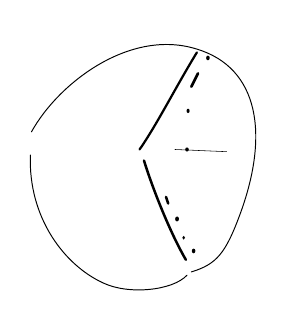
\begin{tikzpicture}[x=.014cm,y=-.014cm,line cap=round,line join=round]
\draw[line width=.35pt] (14,95) .. controls (39,50) and (104,1) .. (164,20) .. controls (220,37) and (230,97) .. (203,170) .. controls (190,205) and (182,215) .. (159,222);
\draw[line width=.35pt] (13,116) .. controls (11,173) and (44,216) .. (79,232) .. controls (102,243) and (142,239) .. (155,225);
\draw[line width=.8pt] (112,111) .. controls (128,88) and (145,54) .. (164,23);
\draw[line width=.9pt] (116,121) .. controls (124,147) and (140,187) .. (154,211);
\fill (174,28) ellipse [x radius=.65pt,y radius=.85pt];
\draw[line width=1pt] (165,42)--(159,54);
\fill (156,76) ellipse [x radius=.55pt,y radius=.8pt];
\draw[line width=.9pt] (136,154)--(138,160);
\fill (146,174) ellipse [x radius=.7pt,y radius=.9pt];
\fill (152,191) ellipse [x radius=.5pt,y radius=.7pt];
\fill (161,203) ellipse [x radius=.65pt,y radius=.85pt];
\draw[line width=.2pt] (144,111)--(191,113);
\fill (155,111) ellipse [x radius=.65pt,y radius=.75pt];
\end{tikzpicture}}
\[ |f(z)|\geq e^{c|z|}|z|^m\prod_i\left|1-\frac z{z_i}\right|\qquad\text{when }-\theta\leq\arg z\leq+\theta \]

On the other hand we have $|f(z)|\leq|h(z)|\leq \mathrm c^{\mathrm{te}}\times e^{\varepsilon|z|}$
whence, supposing that we have chosen $\varepsilon<c$
\[ |z|^m\prod_i\left|1-\frac{z}{z_i}\right|\leq k e^{-\alpha|z|} \]
where $\alpha>0$, whenever $-\theta\leq\arg z\leq+\theta$.

Put $g(z)=z^m\prod_i(1-\frac z{z_i})$, our formula
is written \quad \uline{$|g(z)|\leq ke^{-\alpha|z|}$} \quad if $-\theta\leq\arg z\leq+\theta$

Let us show that \deleted{such} an inequality is possible
for a function $g$ of genus zero only if it
is \deleted{\unsure{identical}} \inserted{constant}. We have indeed also, $g$ being of genus
zero \qquad $|g(z)|\leq k'e^{\frac{\alpha}{3}|z|}$ \qquad for the whole
Put $\omega=e^{\frac{2i\pi}{3}}$, and $G(z)=g(z)g(\omega z)g(\omega^{\unsure{3|2}}z)$
It is an entire function, and one verifies
at once that, \uline{whatever $z$ may be}, we have
\[ |G(z)|\leq(ke^{-\alpha|z|})(k'e^{\frac{\alpha}{3}|z|})(k'e^{\frac{\alpha}{3}|z|})=k''e^{-\frac{\alpha}{3}|z|} \]
\noindent\quad\unsure{!!}

$G(z)$ would therefore be bounded, hence a constant.
But $G(z)=z^{\unsure{-3m|3m}}\prod_i\left(1-\frac{z^3}{z_i^3}\right)$, it
\margin{will be necessary that the set of indices $i$ be empty, and $m=0$, hence
that $g(z)$ be a constant. This means
that $f(z)=\mathrm C^{\mathrm{te}}e^{\beta z}$, which is incompatible
with $|f(z)|\leq|\deleted{\unsure{g}}h(z)|\leq \mathrm c^{\mathrm{te}}e^{\varepsilon|z|}$}
\margin{113}
